% Please make sure you insert your
% data according to the instructions in PoSauthmanual.pdf
\documentclass[a4paper,11pt]{article}
\usepackage{pos}
\usepackage{siunitx}

\title{Recent results in Higgs physics}
%% \ShortTitle{Short Title for header}

\author*[a]{Emanuele Di Marco}
\onbehalf{on behalf of the CMS collaboration}

\affiliation[a]{Istituto Nazionale di Fisica Nucleare (INFN), Sezione di Roma1,\\
  Piazzale Aldo Moro n. 2, 00185, Rome, Italy}

\emailAdd{emanuele.dimarco@roma1.infn.it}

\abstract{This document summarizes recent results from ATLAS and CMS
  collaborations in the measurements of properties and searches of
  Beyond Standard Model effects in Higgs boson physics, using data
  from LHC Runs 2 and 3. The focus is on recent results of
  differential cross section measurements, with their interpretation
  in EFTs, as well analyses probing the CP structure of the couplings
  with vector bosons and tau leptons. Updated measurements of rare
  processes, as $\textrm{H} \to\mu\mu$ or
  $\textrm{H}\to\textrm{Z}\gamma$ are presented, as well as results on
  double or triple Higgs boson productions.  }

\FullConference{The European Physical Society Conference on High Energy Physics (EPS-HEP2025)\\
7-11 July 2025\\
Marseille, France\\}

%% \tableofcontents

\begin{document}
\maketitle


\section{Introduction}

In the ten years since the discovery of the Higgs boson by the
ATLAS~\cite{ATLAS:2008xda,ATLAS:2012yve} and
CMS~\cite{CMS:2008xjf,CMS:2012qbp,CMS:2013btf} Collaborations, much
has been learned about this particle. Most of the major production
modes and decay channels have been observed, and with the
proton-proton collision data collected during Run 2 (2015–2018) and
Run 3 (2022-2024) of the LHC it is possible to probe the cross
sections and properties with increasing precision. The larger datasets
allow access to rare decay modes or rare production processes of the
Higgs boson. Finally, the current data set is used to search for
double Higgs boson production, sensitive to the Higgs self coupling.

\section{Higgs Boson Production and Decay Measurements}

Measurements of Higgs boson production and decay rates were performed
by ATLAS and CMS using up to $140~\text{fb}^{-1}$ of p-p collisions
at $\sqrt{s} = 13~\text{TeV}$ during Run~2 of the LHC, combining the
latest analyses for each process.
%
In the STXS framework, Higgs production is divided into non-overlapping
bins (\emph{STXS bins}) defined by event kinematics. Results are
reported at \textit{stage~0} for major production modes and
\textit{stage~1.2} for finer kinematic subdivisions~\cite{stxs}, and
interpreted in the coupling modifier and \textsc{SMEFT} frameworks~\cite{smeft}.
%
The combination includes $H \to \gamma\gamma$, $ZZ \to 4\ell$, $WW \to
\ell\nu\ell\nu$, $\tau\tau$, $b\bar{b}$, $\mu\mu$, $Z\gamma$, and $H
\to \text{invisible}$ channels, targeting ggH, VBF, VH, ttH, and tH
production.  Off-shell Higgs analyses constrain the total decay width
directly.
%
The overall signal strength $\mu$ is consistent with the Standard
Model (SM) within 5–6\%, dominated by theoretical uncertainties. STXS
measurements are consistent with the SM within 6–18\%, with
significant improvements in $WH$, $ZH$, and $t\bar{t}H+tH$
uncertainties of 30\%, 20\%, and 40\%, respectively.
%
ATLAS measures branching fractions for the main decays ($\gamma\gamma$,
$ZZ^*$, $WW^*$, $b\bar{b}$, $\tau\tau$) with 8–13\% uncertainties,
consistent with SM predictions. Relative improvements of 10–20\% are
achieved in $b\bar{b}$, $WW^*$, and $\tau\tau$ channels, with 29
cross-section $\times$ branching ratio combinations reported.
%
Coupling modifier interpretations yield 5–12\% uncertainties for $W$,
$Z$, $t$, $b$, and $\tau$ couplings, and 25\% for the muon. The charm
coupling is constrained with $^{+1.6}_{-3.8}$, roughly doubling
previous precision.
%
The measured production cross-sections, assuming SM branching
fractions, are shown in Fig.~\ref{fig:stxs} (left), while CMS
performs the most granular fit with 97 parameters of interest, one per
branching ratio in each STXS bin~\cite{cms-comb}, also shown in
Fig.~\ref{fig:stxs} (right).
%
\begin{figure}[!htbp]
\centering
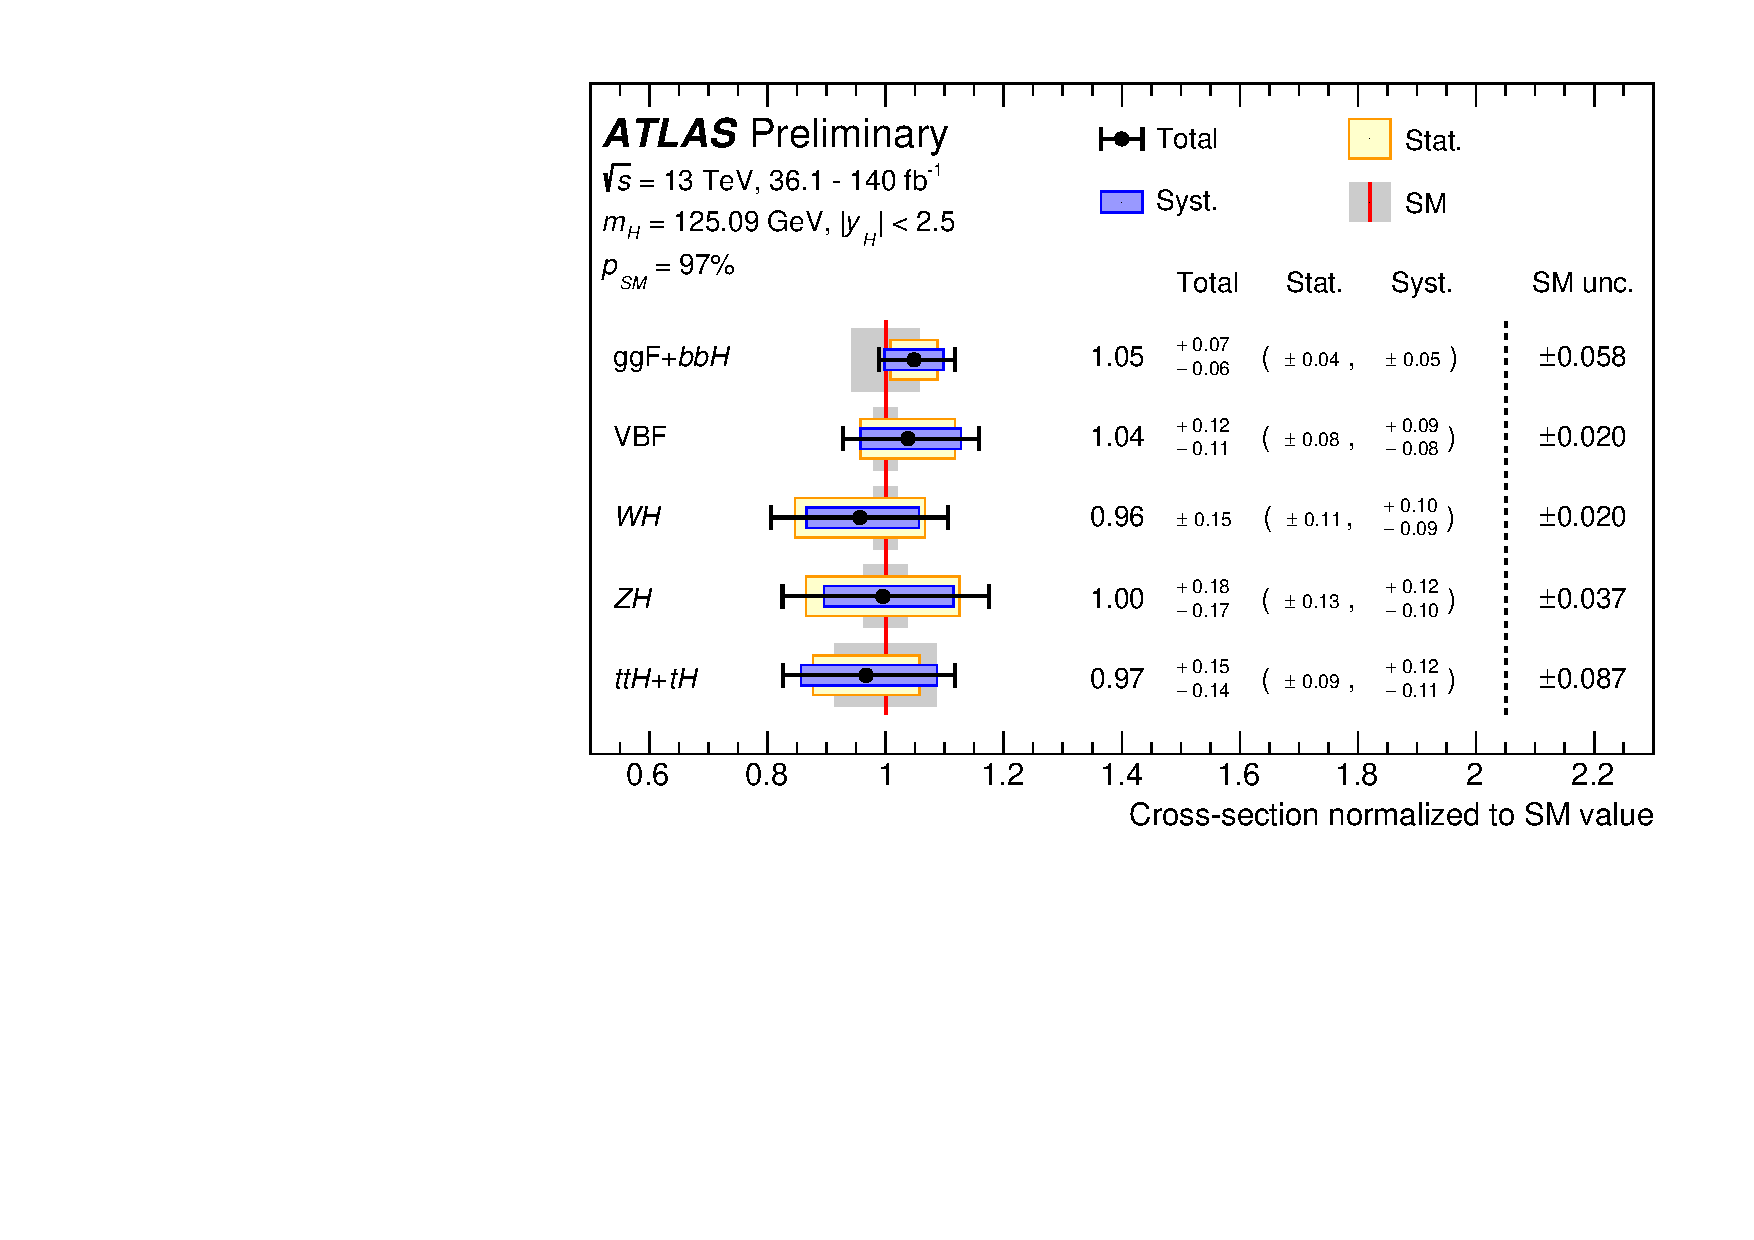
\includegraphics[width=0.45\textwidth]{stxs-atlas-xsecs}
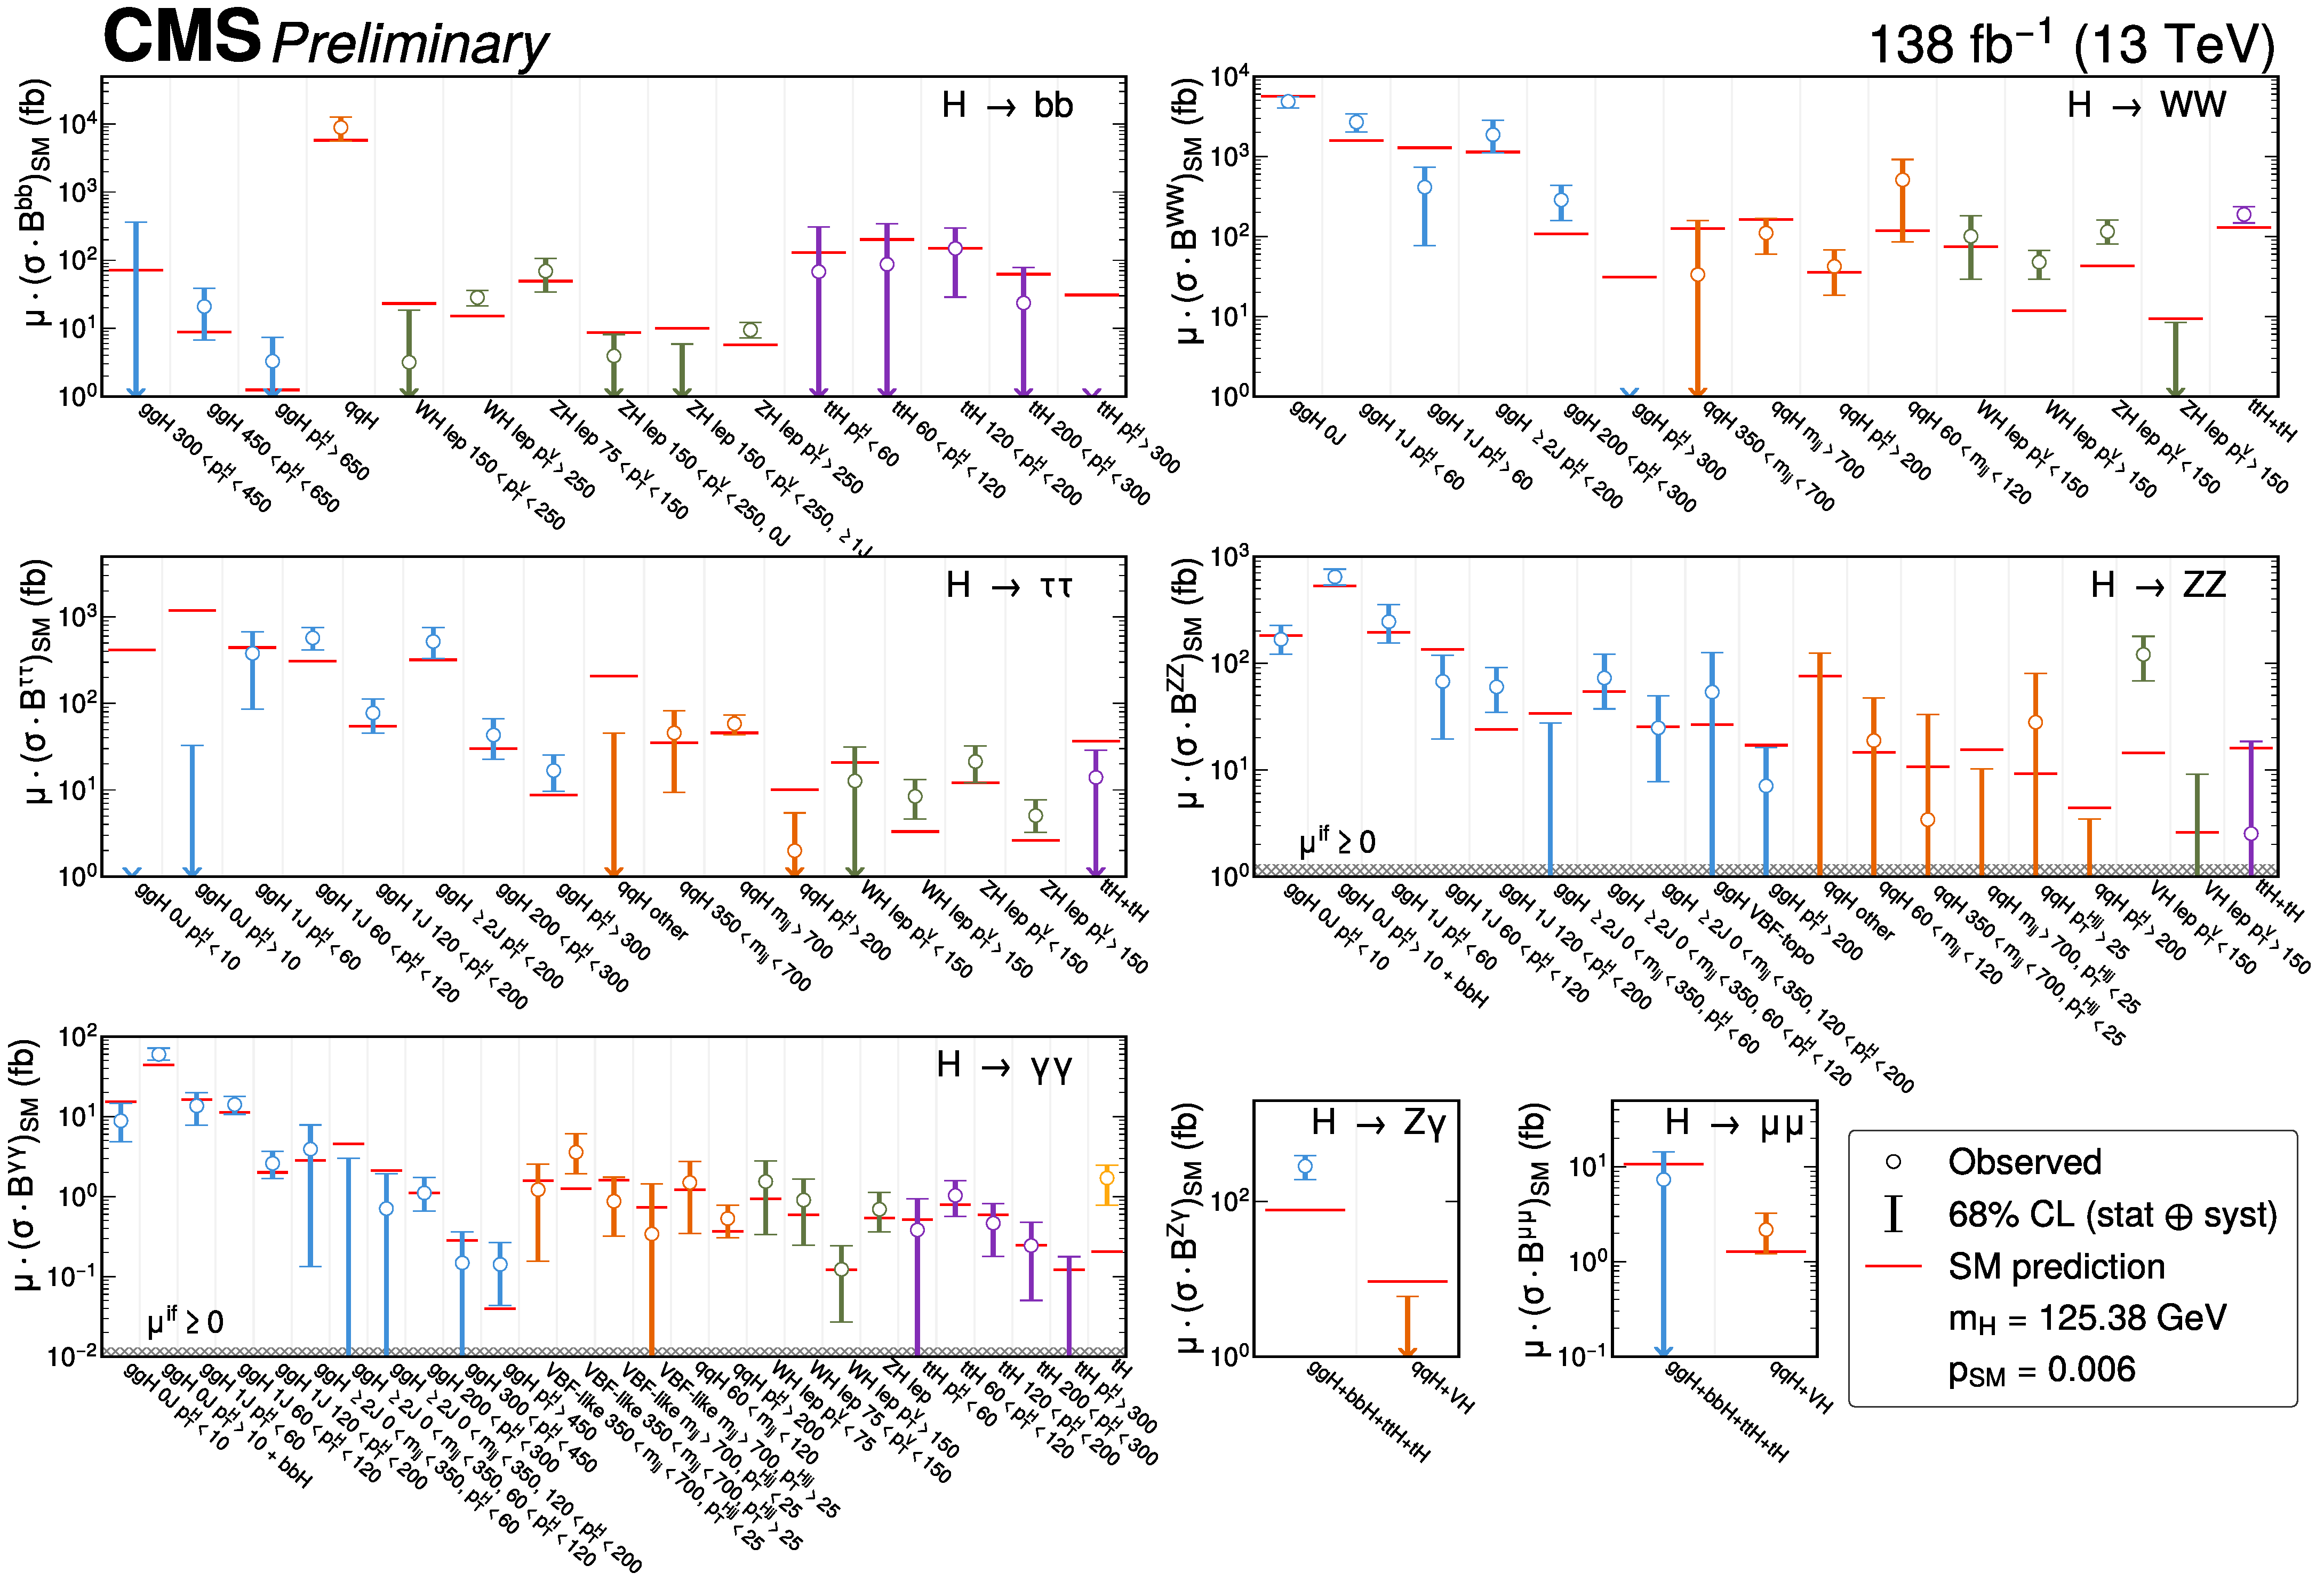
\includegraphics[width=0.45\textwidth]{stxs-cms-xsecs}
\caption
    {Left: observed cross sections values for the main Higgs boson
      production modes, relative to their SM predictions, as measured
      in the most recent ATLAS combination~\cite{atlas-comb}. Right:
      best fit values (white circles) and 68\% CL intervals (coloured
      lines) for the most granular cross section $\times$ branching
      fraction fit in the recent CMS combination~\cite{cms-comb}.
      \label{fig:stxs}
    }
\end{figure}
%
All measurements are found to be in excellent agreement with Standard Model predictions.

\section{Higgs Boson Couplings with Second Generation Fermions}

With the LHC Run 1 and Run 2 data, the Yukawa interactions of the
Higgs boson with third-generation charged fermions have been firmly
established through several measurements involving $\textrm{H}\to b\bar b$ decays. In contrast, the
corresponding coupling to second-generation fermions has not yet been
conclusively observed. Within the SM, the Higgs boson
interactions uniquely distinguish between fermion generations.

\subsection{Higgs decays into two muons}


The decay of the Higgs boson into two oppositely charged muons, $H \to
\mu^+\mu^-$, provides direct sensitivity to the Yukawa coupling of a
second-generation fermion. The SM predicts a branching fraction of
$2.17 \times 10^{-4}$ for this process, for $m_H =
125.09~\mathrm{GeV}$~\cite{yr2}.

An earlier CMS measurement in this channel provided an observed
(expected) significance of $3.0\sigma$ ($2.5\sigma$). The new search
from ATLAS presented here used data recorded during the LHC Run 3,
corresponding to an integrated luminosity of $\SI{165}{fb^{-1}}$ at
$\sqrt{s}=\SI{13.6}{TeV}$, and then combined with the results from Run
2~\cite{hmumu-atlas}.  The reconstruction of this final state relies on the
identification of muons originating from the $H \to \mu^+\mu^-$ decay,
as well as additional particles produced in association with the Higgs
boson candidate. These include other muons, electrons, photons, jets,
and neutrinos, the latter being inferred from the presence of missing
transverse momentum, $p_\mathrm{T}^{\text{miss}}$. The main event
selection requirements are designed to ensure accurate reconstruction
and optimal separation of signal and background processes.

Events passing the baseline selection are classified into 23 exclusive
categories optimized to distinguish between background processes and
the various Higgs boson production mechanisms: $t\bar{t}H$, $VH$, VBF,
and ggF. Multivariate classifiers are employed to enhance signal
sensitivity, utilising variables exploit the kinematic properties
of final-state particles.
%
The dominant background arises from Drell--Yan production, with
additional contributions from diboson, $t\bar{t}$, single-top, and
rarer electroweak processes. Background normalization is determined
from data sidebands in $m_{\mu\mu}$ =
\qtyrange[range-phrase=~--~]{110}{120}{GeV} and
\qtyrange[range-phrase=~--~]{130}{160}{GeV}. Signal extraction is
performed using a binned maximum-likelihood fit to the $m_{\mu\mu}$
distribution in the range
\qtyrange[range-phrase=~--~]{110}{160}{GeV}. The signal is modeled by
a double-sided Crystal Ball function with a mass resolution of
\qtyrange[range-phrase=~--~]{2.8}{3.2}{GeV}. The observed mass
spectrum, together with the superimposed likelihood fit, is shown in
Fig.~\ref{fig:gen2f} (left).
%% Systematic uncertainties include
%% theoretical cross-section and PDF uncertainties, and experimental
%% effects related to muon efficiencies, energy/momentum scale, jet
%% calibration, pile-up, and luminosity.
%
The dominant systematic uncertainty arises from background modeling,
followed by theoretical and muon-related sources. The fit to the
observed $m_{\mu\mu}$ spectra yields a best-fit signal strength of
$\mu = 1.6 \pm 0.6$, corresponding to an observed (expected)
significance of 2.8 (1.8)\,$\sigma$. Combining these results with the
full Run~2 dataset increases the observed (expected) significance to
3.4 (2.5)\,$\sigma$, corresponding to a branching fraction of $
\mathcal{B}(H \to \mu^+\mu^-) = (3.0 \pm 0.9) \times 10^{-4}$,
consistent with the SM expectation.

\subsection{Higgs decays into c quark pairs}

A search for Higgs boson decays into a charm quark--antiquark pair,
$H\to c\bar{c}$, has been performed by CMS using the full LHC Run 2
data~\cite{tthcc-cms}. The analysis targets Higgs boson production in
association with a top quark pair ($t\bar{t}H$), performed
simultaneously with the measurement of $H\to b\bar{b}$. The analogous
$t\bar{t}Z$ processes with $Z\to c\bar{c}$ and $Z\to b\bar{b}$ decays
are used for validation. The event reconstruction employs advanced
machine learning algorithms, including
\textsc{ParticleNet}~\cite{pnet} for jet flavour identification and
the \textsc{Particle Transformer}~\cite{ptran} for event
classification. Events are categorized according to lepton
multiplicity and heavy-flavour content to enhance signal purity.
%
Backgrounds from $t\bar{t}+$jets, $t\bar{t}W$, and single-top
production are modelled using NLO simulations with flavour-dependent
corrections constrained by control regions in data. Signal extraction
is performed via a simultaneous binned likelihood fit to the
\textsc{Particle Transformer} discriminants. The measured signal
strengths are $\mu_{t\bar{t}H(H\to b\bar{b})}=0.91^{+0.26}_{-0.22}$
and $\mu_{t\bar{t}H(H\to c\bar{c})}=-1.6\pm4.5$, with an observed
(expected) significance of 4.4 (4.5)\,$\sigma$ for $t\bar{t}H(H\to
b\bar{b})$. No excess is observed in the $t\bar{t}H(H\to c\bar{c})$
channel, leading to an observed (expected) 95\% confidence level upper
limit of $\mu_{t\bar{t}H(H\to c\bar{c})}<7.8~(8.7^{+4.0}_{-2.6})$.

Combining this result with previous searches in the $VH$ production
mode yields the most stringent constraint to date on the charm Yukawa
coupling, with an observed (expected) 95\% CL bound of
$|\kappa_c|<3.5~(2.7)$, assuming SM production cross sections. The
corresponding upper limits in the two production modes, as well as
their combination are shown in Fig.~\ref{fig:gen2f} (right).

\begin{figure}[!tbp]
\centering
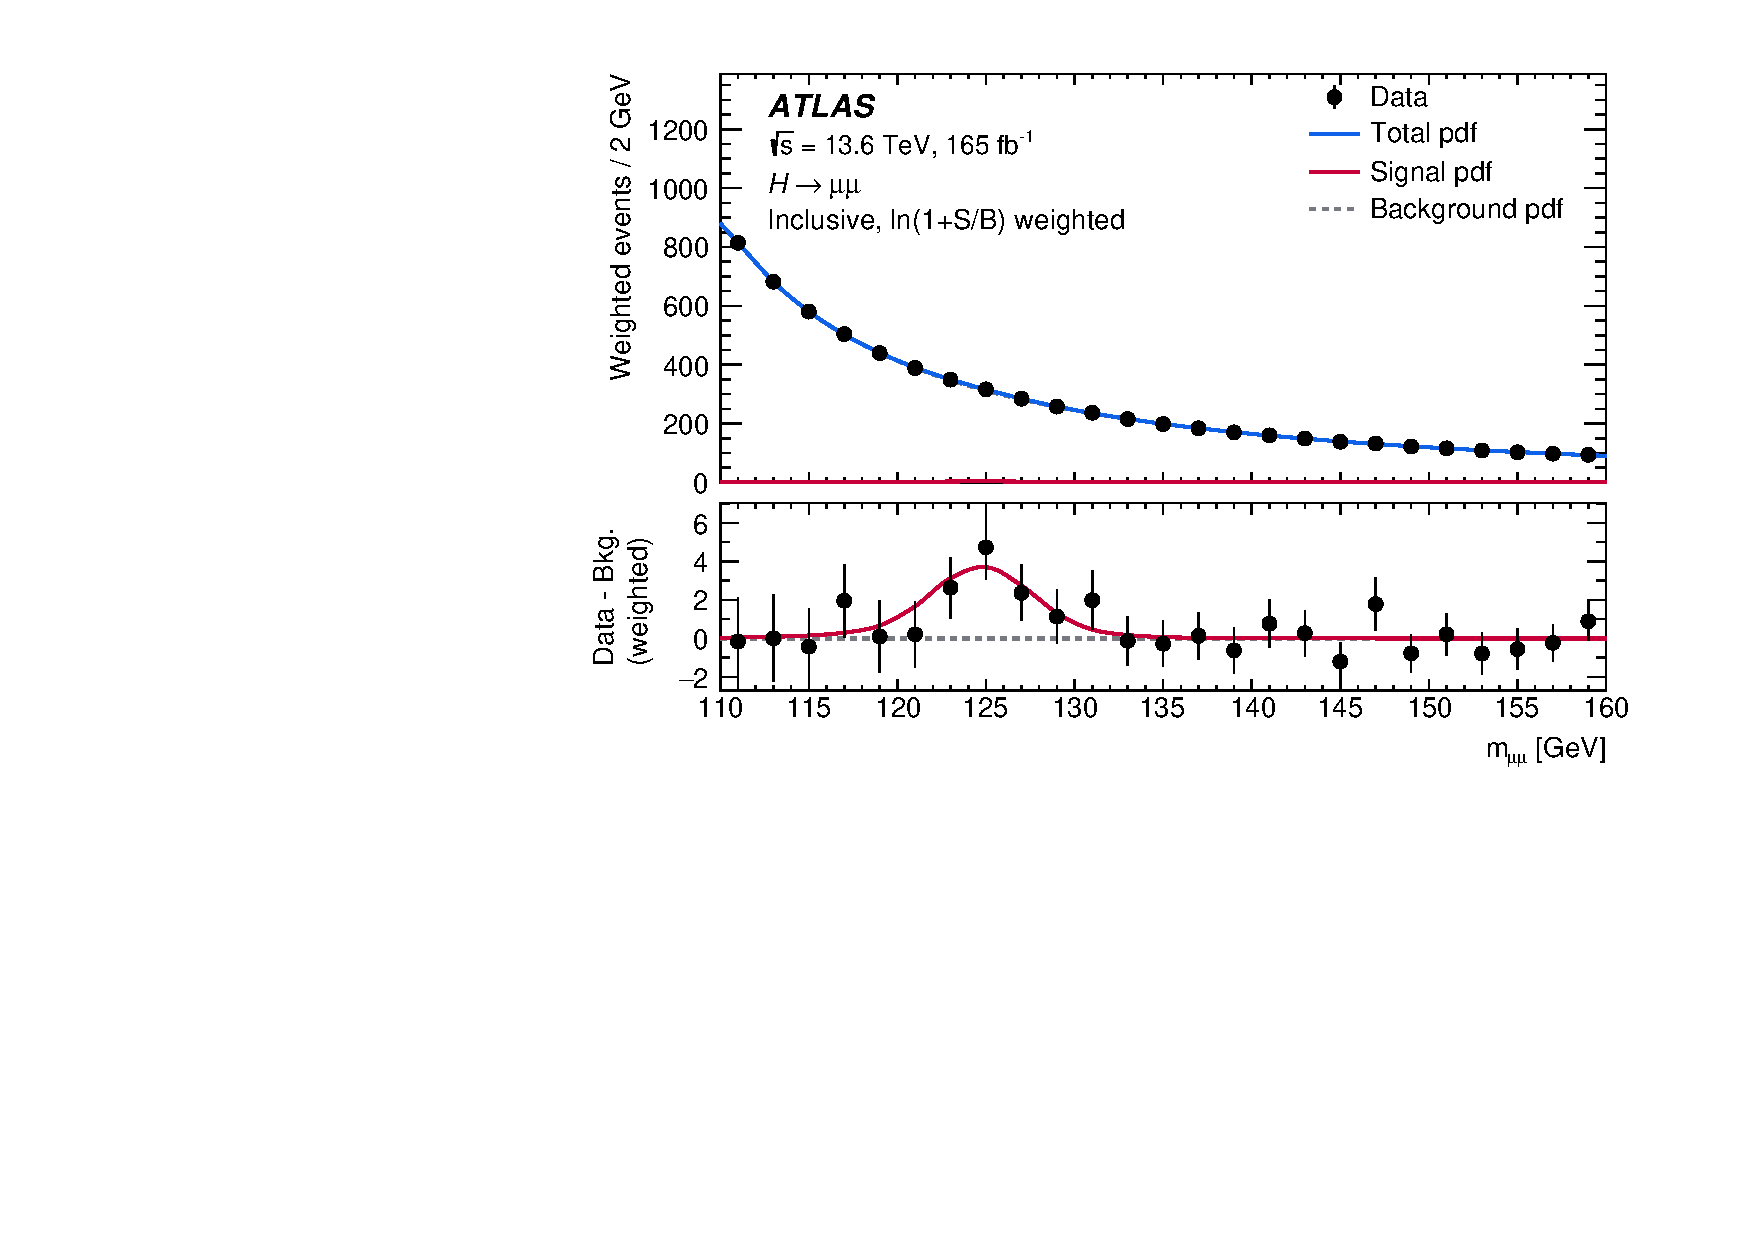
\includegraphics[width=0.45\textwidth]{hmumu-atlas}
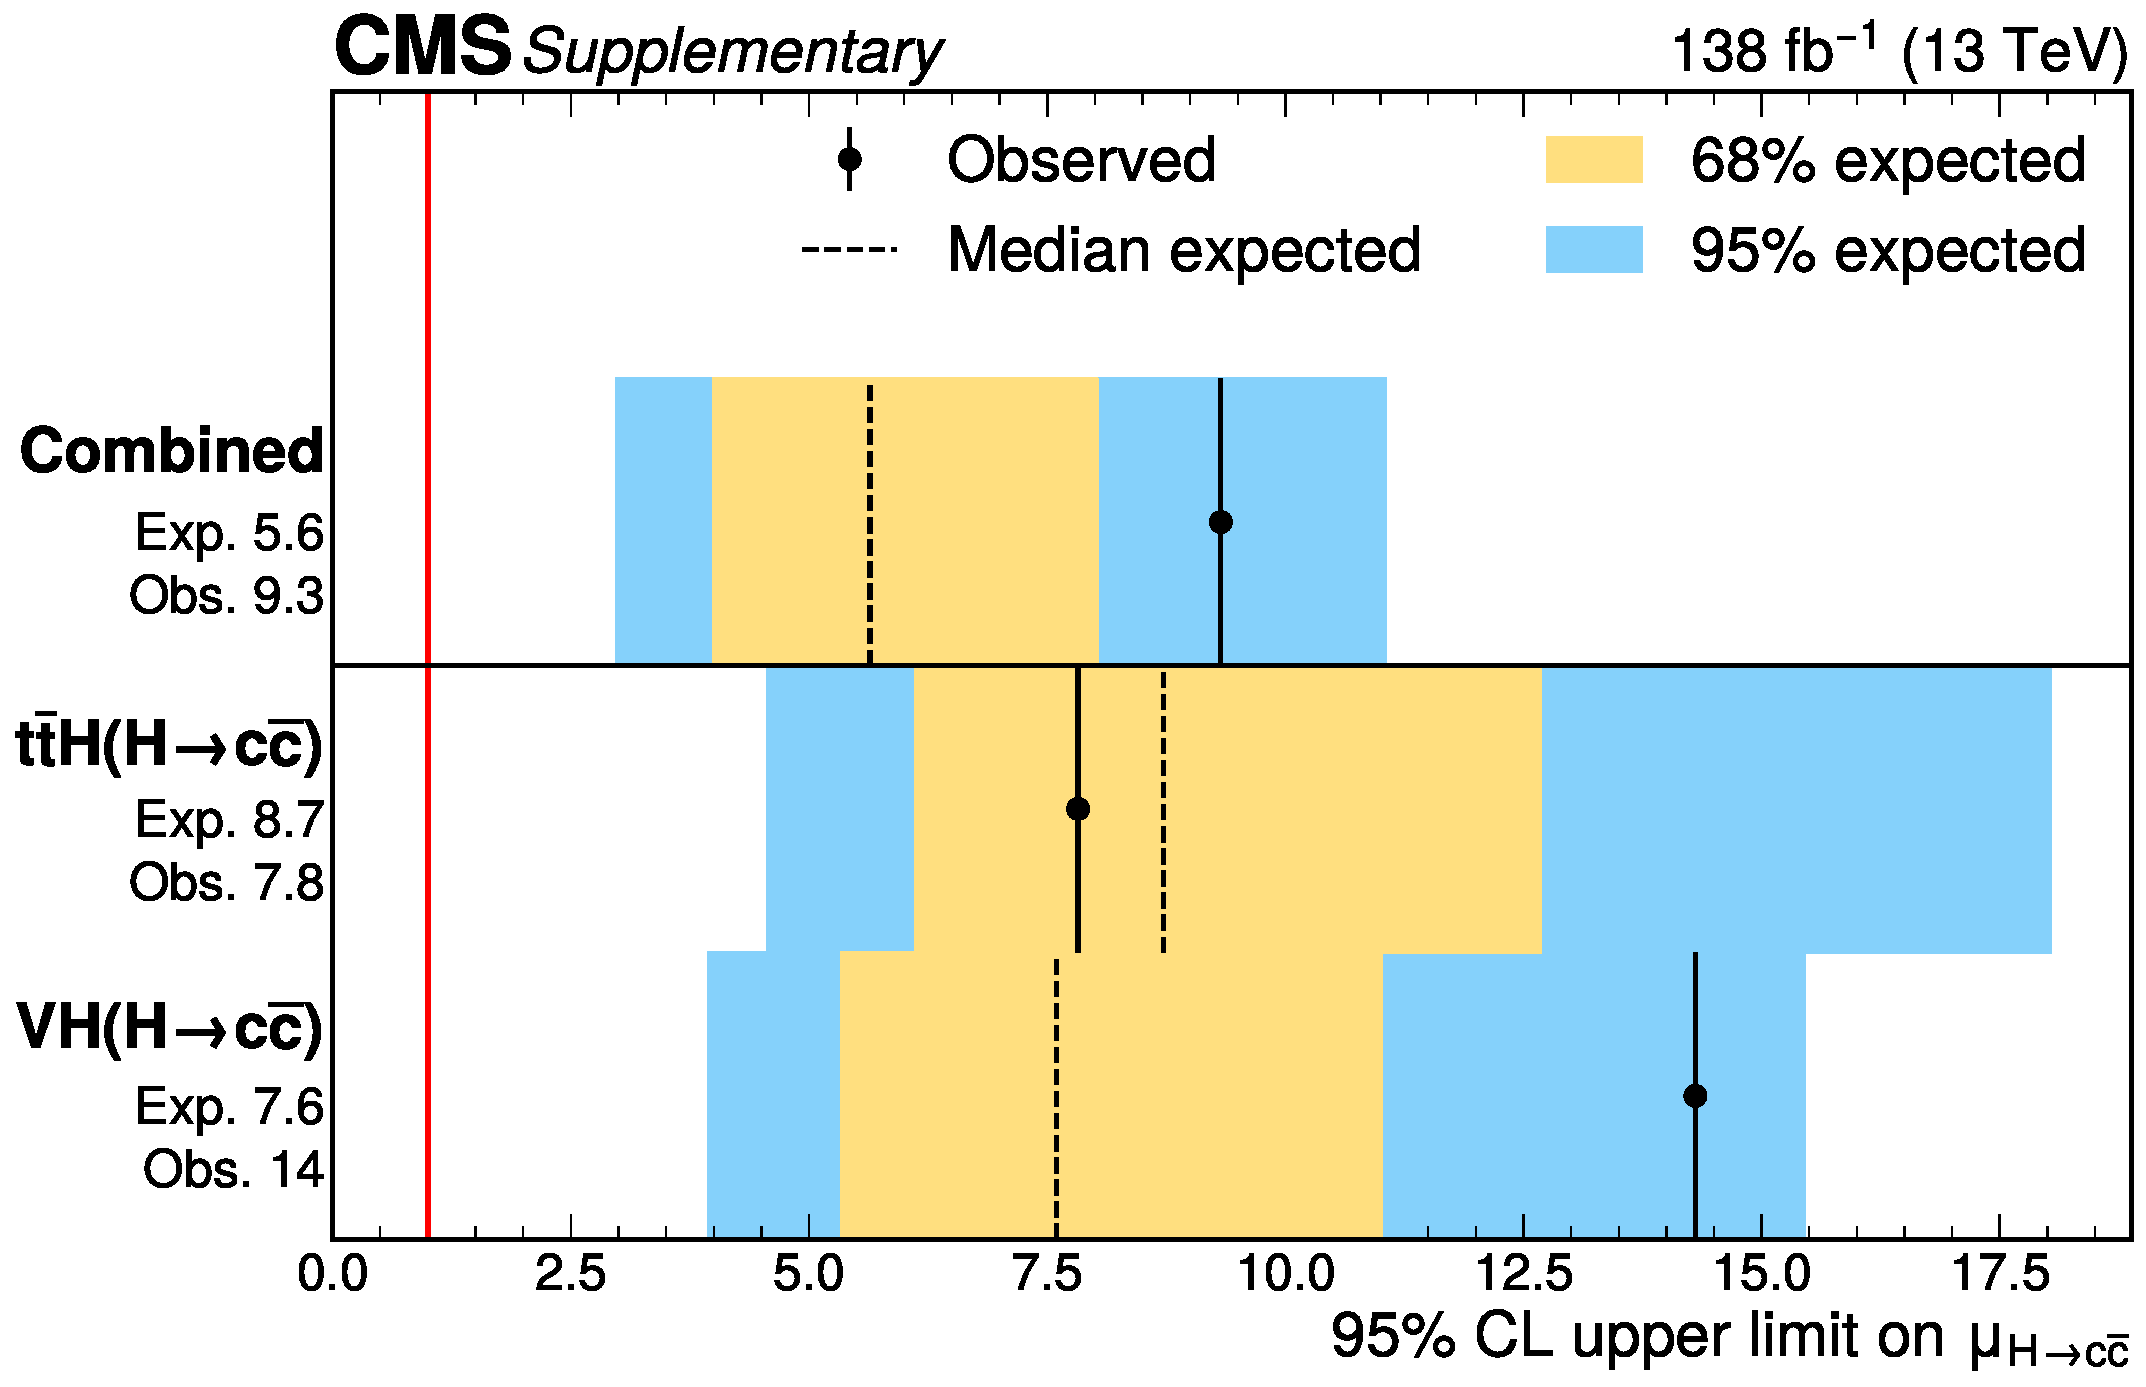
\includegraphics[width=0.45\textwidth]{ttHcc-cms}
\caption
    {Left: S/B weighted observed dimuon invariant mass spectrum in the
      ATLAS Run 3 data, combining all analysis
      categories~\cite{hmumu-atlas}. Right: the 95\% CL upper limits on
      $\mu_{t\bar t H(H\to c\bar c)}$ for the CMS analysis~\cite{tthcc-cms}. The blue
      and yellow bands indicate the expected 68\% and 95\% CL regions,
      respectively, under the background-only hypothesis.
      \label{fig:gen2f}
    }
\end{figure}

\section{Rare decay channels and production modes}

\subsection{Decay Into a Z Boson and a Photon}

Within the SM, the Higgs boson decay to a $Z$ boson and a photon ($H
\to Z\gamma$) occurs via loop-induced processes, yielding a predicted
branching ratio of BR($H \to Z\gamma$) = $(1.54^{+0.10}_{-0.11})
\times 10^{-3}$ for $m_H = 125.09$~GeV, similar to $H \to
\gamma\gamma$. Extensions of the SM can modify this rate through new
particles in the loops, making the ratio BR($H \to Z\gamma$)/BR($H \to
\gamma\gamma$) a sensitive probe of new physics. Observation of $H \to
Z\gamma$ would complete the set of Higgs decays into electroweak boson
pairs, consolidating its role in electroweak symmetry breaking. The
$Z(\to \ell\ell)\gamma$ final state ($\ell=e,\mu$) offers the best
sensitivity, providing full kinematic reconstruction and excellent
invariant-mass resolution.

The earlier combination of ATLAS and CMS Run-2 searches at
$\sqrt{s}=13$~TeV with 140~fb$^{-1}$ yielded a first evidence for $H
\to Z\gamma$ at 3.4\,$\sigma$, $\mu = 2.2 \pm 0.7$. The results
presented here include a Run-3 search using \SI{165}{fb^{-1}} at
$\sqrt{s}=\SI{13.6}{TeV}$~\cite{hzgamma-atlas}. Improvements include
increased production cross-section, larger datasets, optimized $p_T$
thresholds, and 13 event categories, including a new multi-lepton
category. Twelve categories use an improved multivariate classifier to
enhance sensitivity. A simultaneous fit to the $Z\gamma$ invariant
mass across all categories extracts the $H \to Z\gamma$ signal, which
is combined with Run-2 results to further increase sensitivity.
%
The $H\to Z\gamma$ signal is extracted via an unbinned
maximum-likelihood fit to $m_{Z\gamma}$ distributions across all Run-3
categories, including nuisance parameters for systematic
uncertainties.  The measured signal strength is $\mu =
0.9^{+0.7}_{-0.6}$, compatible with the SM expectation $\mu_{\rm exp}
= 1.0\pm0.7$, with observed (expected) significance 1.4
(1.5)\,$\sigma$.  Statistical uncertainties dominate, while background
modelling is the largest systematic.  Run-3 improves expected
significance by 28\% relative to Run-2, due to optimized selection,
categorisation, and larger dataset at $\sqrt{s}=13.6$ TeV.  Run-3
results are combined with Run-2, correlating theoretical but not most
of the experimental uncertainties.  The combined fit gives $\mu =
1.3^{+0.6}_{-0.5}$ with a significance of 2.5\,$\sigma$ ($1.9\,\sigma$
expected), compatible with Run-2 (p-value=0.33).  This provides the
most stringent sensitivity to date for $H\to Z\gamma$ branching
fraction.  Assuming SM production, the observed branching fraction is
$(2.0^{+0.9}_{-0.8})\times 10^{-3}$, consistent with the SM prediction
of $(1.54^{+0.10}_{-0.11})\times 10^{-3}$.


\subsection{Electroweak VVH production}

VVH production via vector boson scattering (VBS) probes the Higgs
self-coupling ($\kappa_\lambda$) and VVHH quartic coupling
($\kappa_{2V}$), with a SM LO cross section of \SI{1.77}{fb} at
$\sqrt{s} = \SI{13}{TeV}$.  The search~\cite{vvhbb-cms} uses 138
fb$^{-1}$ of CMS data (2016--2018), targeting $H \to b\bar{b}$ decays
in all-hadronic, semileptonic, and dileptonic channels.  Higgs boson
and vector boson decay products are reconstructed as large-cone jets,
with forward-backward VBS jet pairs exploited.  Channel orthogonality
is ensured via lepton and jet multiplicities, $Z$ mass windows, and
specific selections; multivariate techniques (DNNs, BDTs) are used for
signal discrimination.  Backgrounds are estimated through
extrapolation from control regions; signal extraction uses simple
counting in the signal region, subtracting the background prediction.
Systematic uncertainties include factorization/renormalization scales,
PDFs, jet/lepton reconstruction, b-tagging, boosted resonance tagging,
and integrated luminosity.  The 95\% CL intervals are $\kappa_{2V} \in
[0.40, 1.60]$, $\kappa_{2W} \in [0.17, 1.84]$, $\kappa_{2Z} \in
[-0.37, 2.38]$, with two-dimensional likelihood scans further
constraining anomalous quartic couplings, as shown in
Fig.~\ref{fig:rare} (right).



\begin{figure}[!tbp]
\centering
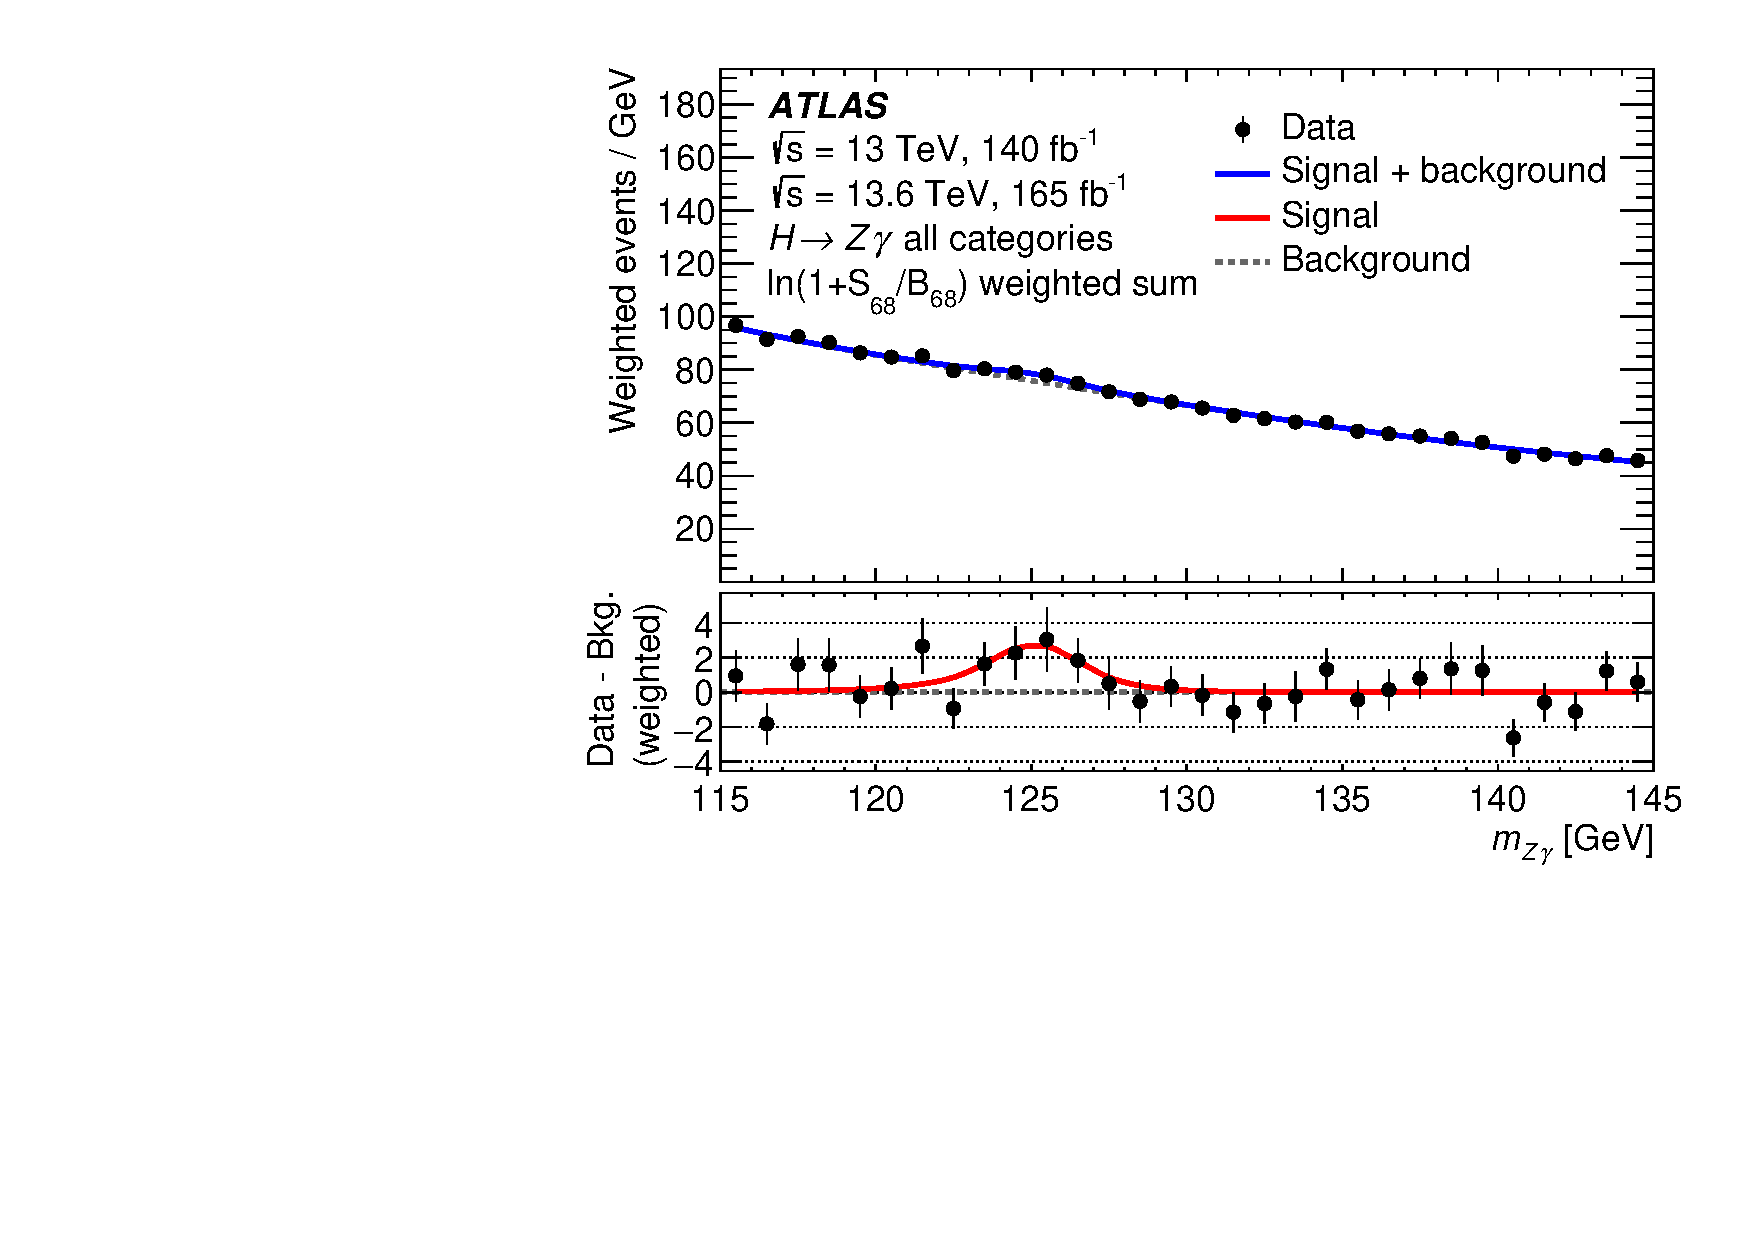
\includegraphics[width=0.45\textwidth]{hzgamma-atlas}
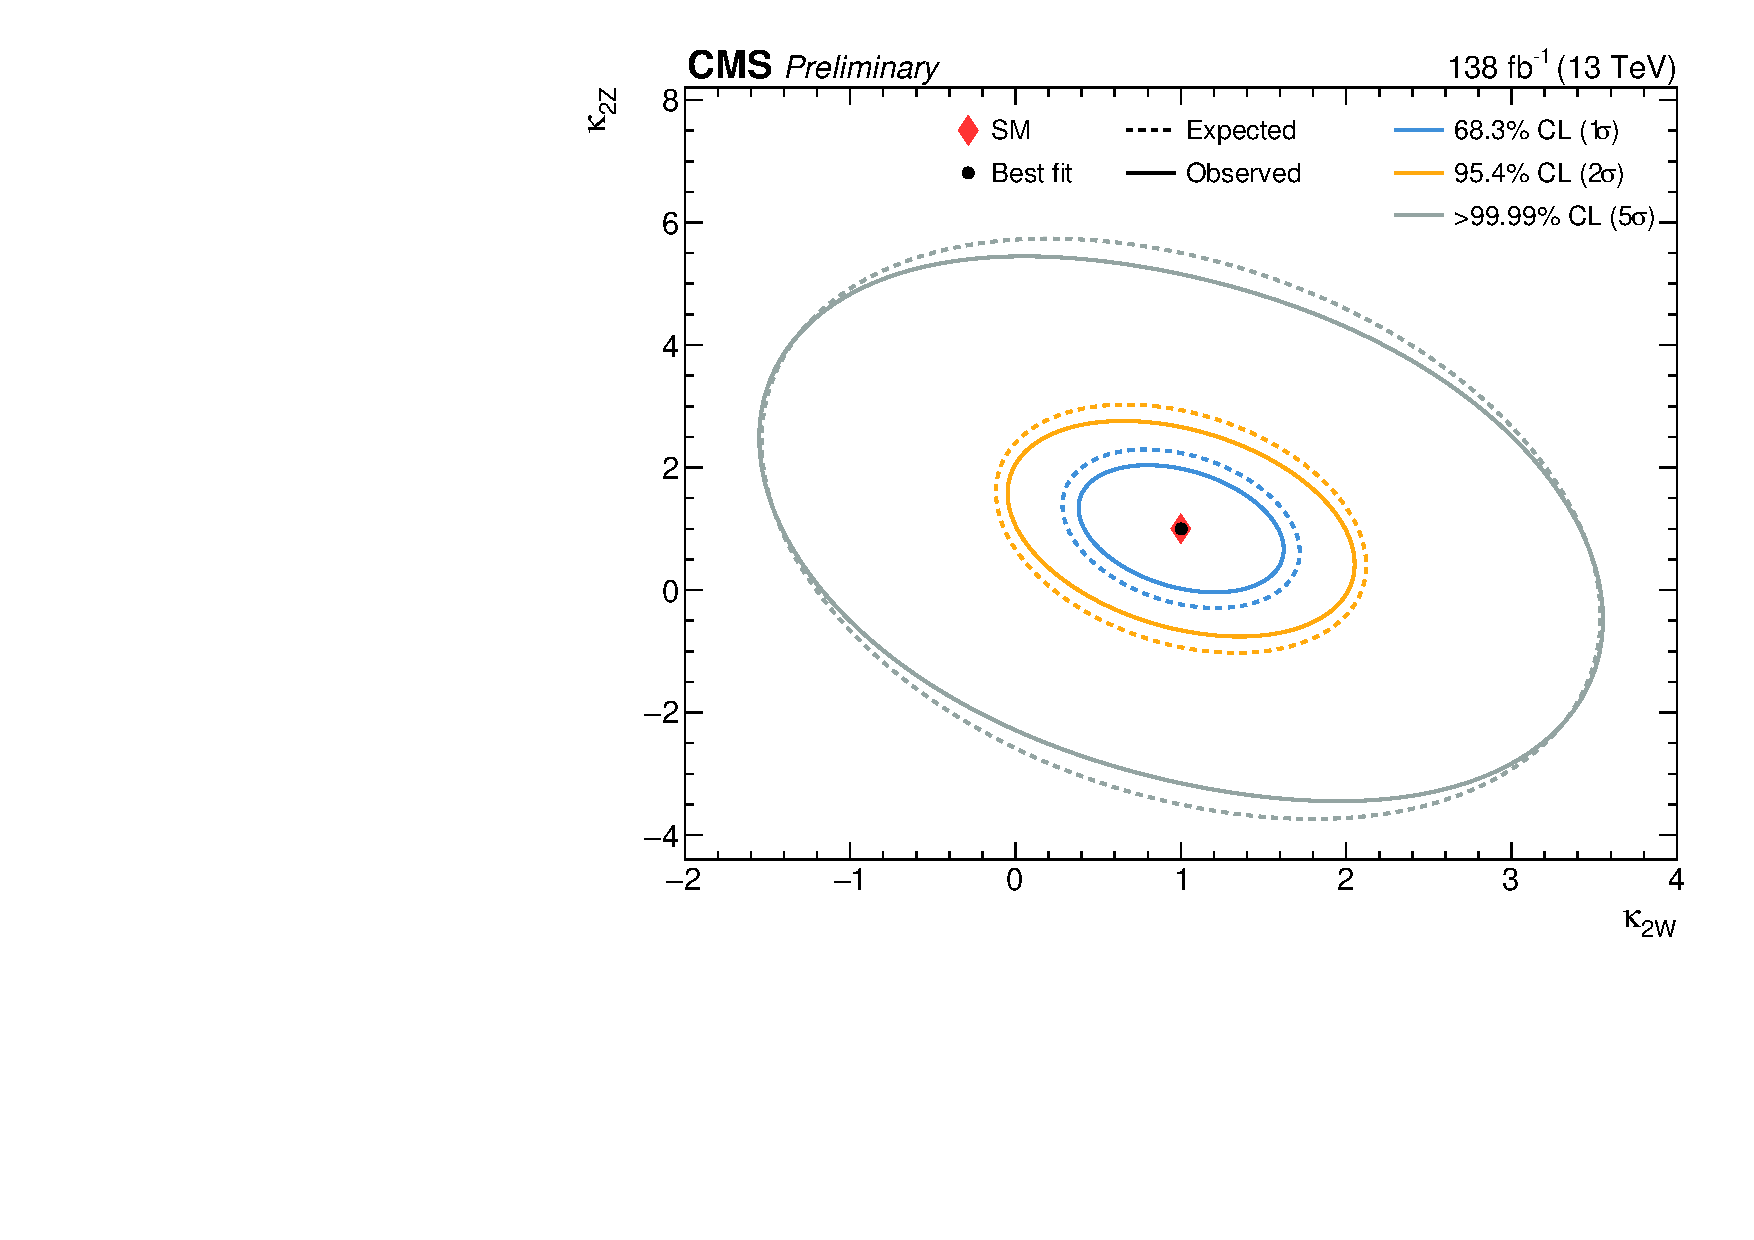
\includegraphics[width=0.45\textwidth]{vvhbb-cms}
\caption
    {Left: $Z\gamma$ invariant mass distributions of S/B weighted data
      for the combined Run-2 and Run-3 ATLAS
      dataset~\cite{hzgamma-atlas}. The black points represent the
      data, while the signal-plus-background fit (solid blue curve)
      and the background model (dashed line) are overlaid.  Right:
      observed (solid line) and expected (dashed line) 1, 2 and 5
      $\sigma$ exclusion regions in the $\kappa_{2W}-\kappa_{2Z}$
      plane from the CMS $VVH(H \to b\bar b)$ analysis using Run-2
      data~\cite{vvhbb-cms}.
      \label{fig:rare}
    }
\end{figure}

\section{CP Properties}

The Higgs boson spin-parity is consistent with $J^{PC}=0^{++}$,
excluding nonzero spin assignments, though small anomalous couplings
to electroweak bosons ($HVV$) or gluons ($Hgg$) remain possible.
CP-violating effects in Higgs boson couplings to fermions ($Hff$) and
gluons, probed via $ttH$ production and $H \to \tau\tau$ decays,
provide complementary insights and indirect searches for BSM
phenomena, with current constraints limited in sensitivity.  New
results on this topic are presented here, using $H\to\gamma\gamma$ decay
channel (CMS) and $H\to\tau^+\tau^-$ channel (ATLAS), using the LHC
Run 2 data.

\subsection{Anomalous Higgs Boson Couplings in $H\to\gamma\gamma$ Decay}

In the CMS analysis of the $H \to \gamma\gamma$
channel~\cite{hggac-cms}, the formalism of previous CMS analyses is
adopted to study anomalous Higgs boson couplings in HVV and Hgg
interactions.  The HVV amplitude is described by three tensor
structures with coefficients expanded in $q^2/\Lambda^2_1$, including
potential CP-odd contributions~\cite{Gao:2010qx}. In the SM, only the
tree-level contributions proportional to $a_1$ are nonzero, with other
couplings considered anomalous or loop-induced.  CP-odd terms $a_3$
lead to CP violation when combined with CP-even couplings.  Effective
fractional cross sections $f_{ai}$ are measured instead of direct
couplings, canceling many uncertainties. The analysis uses $H \to
\gamma\gamma$ decays, measuring one anomalous coupling at a time, and
optionally up to four simultaneously.

The sensitivity to HVV couplings is obtained from VBF and VH
production, with preselected events categorized to enhance signal
discrimination, though ggH and ttH events also populate these
categories. VBF categories require at least two jets with $m_{jj} >
350$~GeV, leading jet $p_T > 40$~GeV, subleading jet $p_T > 30$~GeV,
and $|\eta| < 4.7$, then divided using dedicated matrix element or
multivariate discriminants, optimized for CP-odd sensitivity. Five VBF
tags retain optimal sensitivity to anomalous couplings $f_{a3}$,
$f_{\Lambda1}$, $f_{Z\gamma}^{\Lambda1}$, and $f_{a2}$, with inputs
including jet kinematics and photon angular variables.
%
$V(\mathrm{had})H$ categories select two jets with $60 < m_{jj} <
120$~GeV and use a DNN outputs to define five categories, including
two BSM-dominated tags. $V(\mathrm{lep})H$ categories target
$Z(\ell\ell)H$, $W(\ell\nu)H$, and $Z(\nu\nu)H$ events, using lepton
and $p_\mathrm{T}^{\text{miss}}$ selections combined with STXS and
BSM-trained BDTs.  Expected signal and background yields are
determined for each category, with high-purity tags targeting maximal
anomalous coupling contributions. This categorization strategy allows
a simultaneous fit across all reconstructed categories, constraining
both SM and BSM HVV contributions in situ.
%
The effective cross section ratios \(\vec{f} = f_{a2}, f_{a3},
f_{\Lambda 1}, f^{Z\gamma}_{\Lambda 1}\) are extracted via a
simultaneous fit to the \(m_{\gamma\gamma}\) distributions across all
categories.  In the HVV analysis, constraints are placed on the
CP-violating parameter \(f_{a3}\) and CP-conserving parameters
\(f_{a2}, f_{\Lambda 1}, f^{Z\gamma}_{\Lambda 1}\).  The resulting
68\% CL limits are \(f_{a3} = (0.00^{+0.39}_{-0.39})\times10^{-4},
f_{a2} = (-0.81^{+0.65}_{-2.0})\times10^{-4}, f_{\Lambda 1} =
(-0.014^{+0.032}_{-0.14})\times10^{-4}, f^{Z\gamma}_{\Lambda 1} =
(0.83^{+1.5}_{-0.92})\times10^{-4}\), representing some of the most
stringent limits to date. One example of the resulting likelihood
curve for the $f_{a3}$ parameter for HVV couplings is shown in
Fig.~\ref{fig:cp} (left).





\subsection{CP in $H\to \tau^+\tau^-$ decay}

ATLAS has performed a search for CP violation in the VBF production of
the Higgs boson using the $H \to \tau^+\tau^-$ decay, which provides a
high signal-to-background ratio and efficient
reconstruction~\cite{httcp-atlas}. The study uses 140~fb$^{-1}$ of
Run~2 $pp$ collisions. The Optimal Observable method, incorporating
full multidimensional production phase space information, is employed,
with additional CP-odd observables used for comparison. The analysis
benefits from updated background estimates and novel machine learning
techniques, with results interpreted in the HISZ and Warsaw bases.
%
Events with at least two jets and a Higgs candidate decaying via
$H\to\tau^+\tau^-$ are targeted. Three $\tau$ decay channels are
considered: fully hadronic ($\tau_{\rm had}\tau_{\rm had}$),
semileptonic ($\tau_{\rm lep}\tau_{\rm had}$), and leptonic
($\tau_{\rm lep}\tau_{\rm lep}$), with same-flavor leptonic decays
rejected to reduce $Z\to ee/\mu\mu$ backgrounds.
%
CP parameters are extracted via a binned maximum-likelihood fit over
SRs and CRs, with signal templates reweighted from SM VBF Higgs
predictions.  Signal regions are binned in the Optimal Observable,
with one CR per SR to constrain $Z\to\tau^+\tau^-$. A common
normalization factor is applied to signal, equal to
($\mu_\mathrm{VBFH}=0.87^{+0.14}_{-0.13}$) as well as for the
background, with top background constrained in the leptonic
channel. Fits are performed separately for each decay channel and
combined, treating experimental and theoretical uncertainties as
correlated.
%
No significant deviation from the SM CP-even Higgs boson is
observed. The parameter $\tilde{d}$ is constrained to
$[-0.012,+0.044]$, and the parameter $c_{H\tilde{W}}$ to
$[-0.24,+0.83]$ for the BSM scale $\Lambda = 1$~TeV, including linear
and quadratic terms. These results are competitive with other decay
modes, such as $H\to ZZ^*$ and $H\to\gamma\gamma$ (Fig.~\ref{fig:cp},
right).



\begin{figure}[!htbp]
\centering
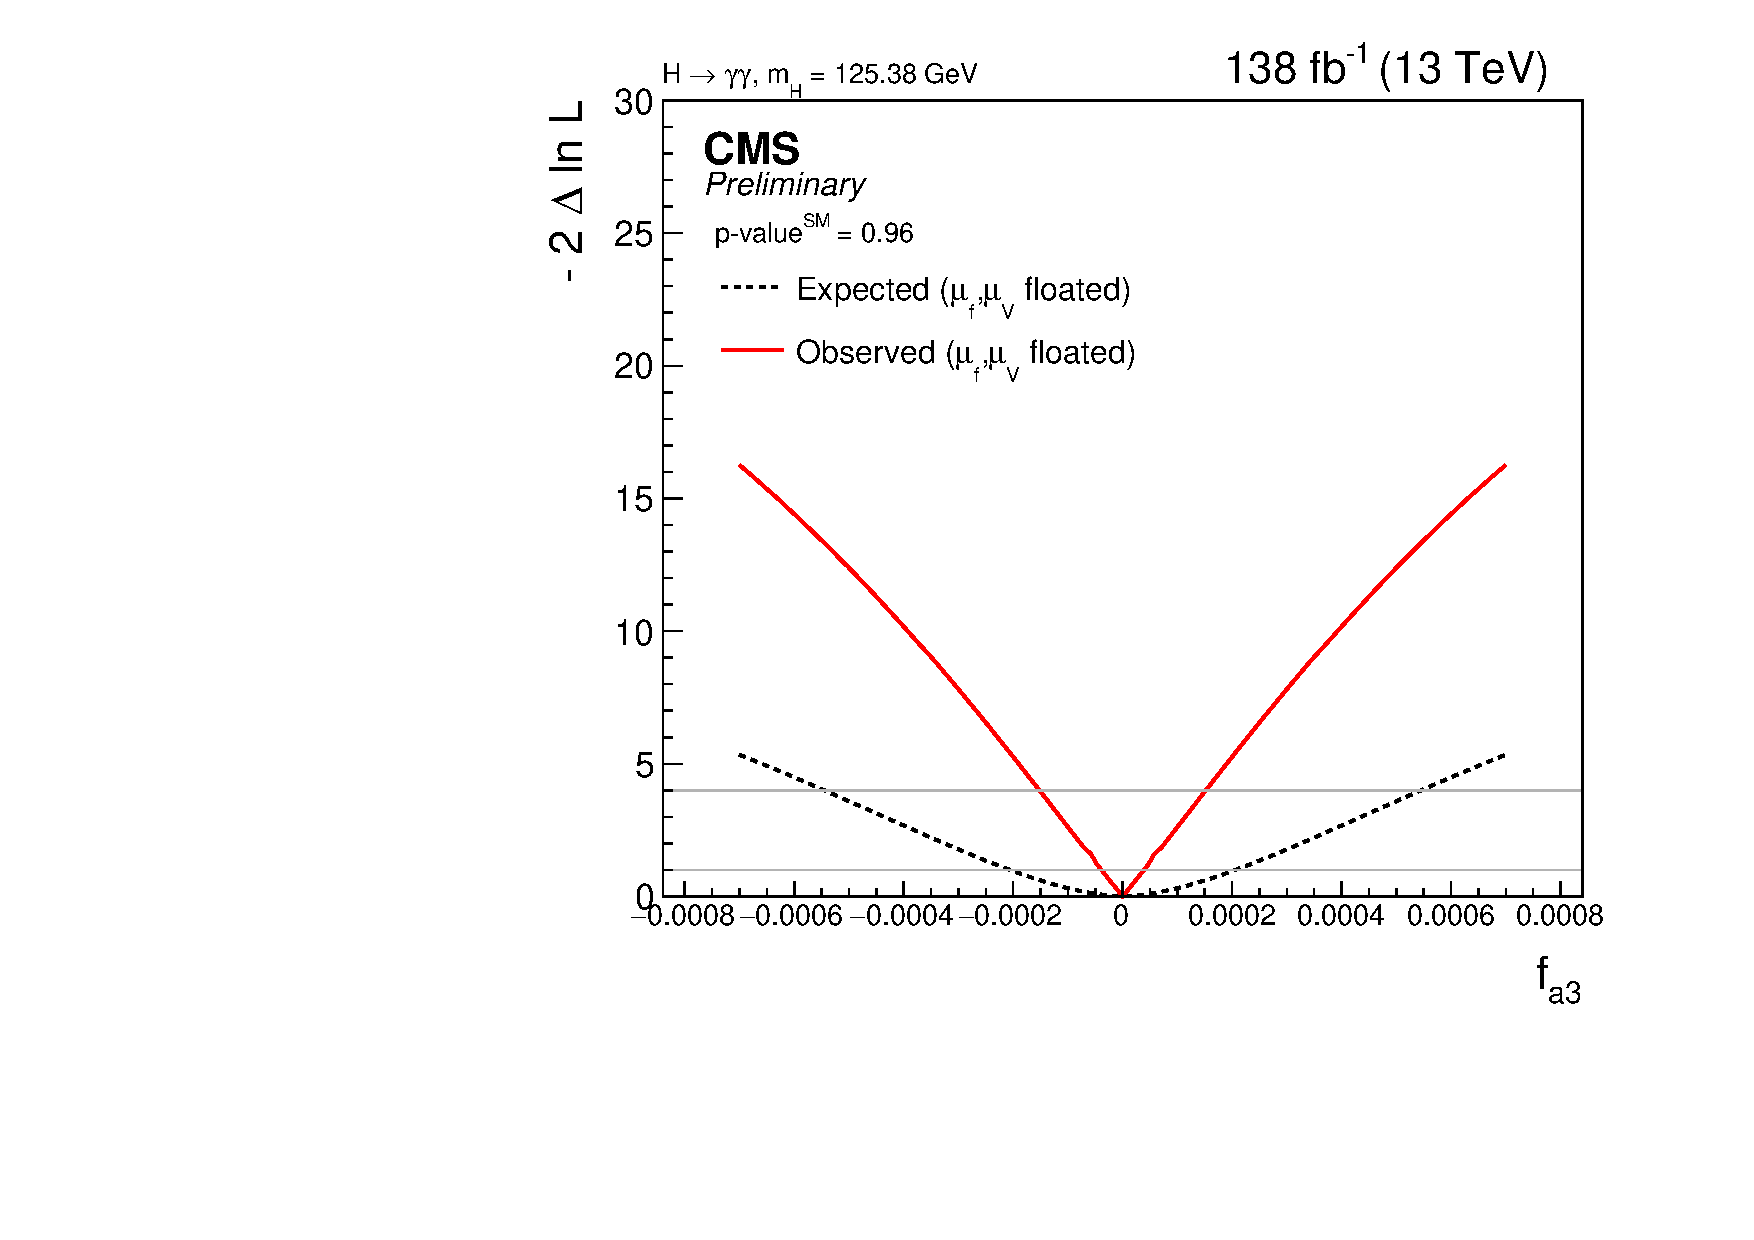
\includegraphics[width=0.45\textwidth]{fa3-cms}
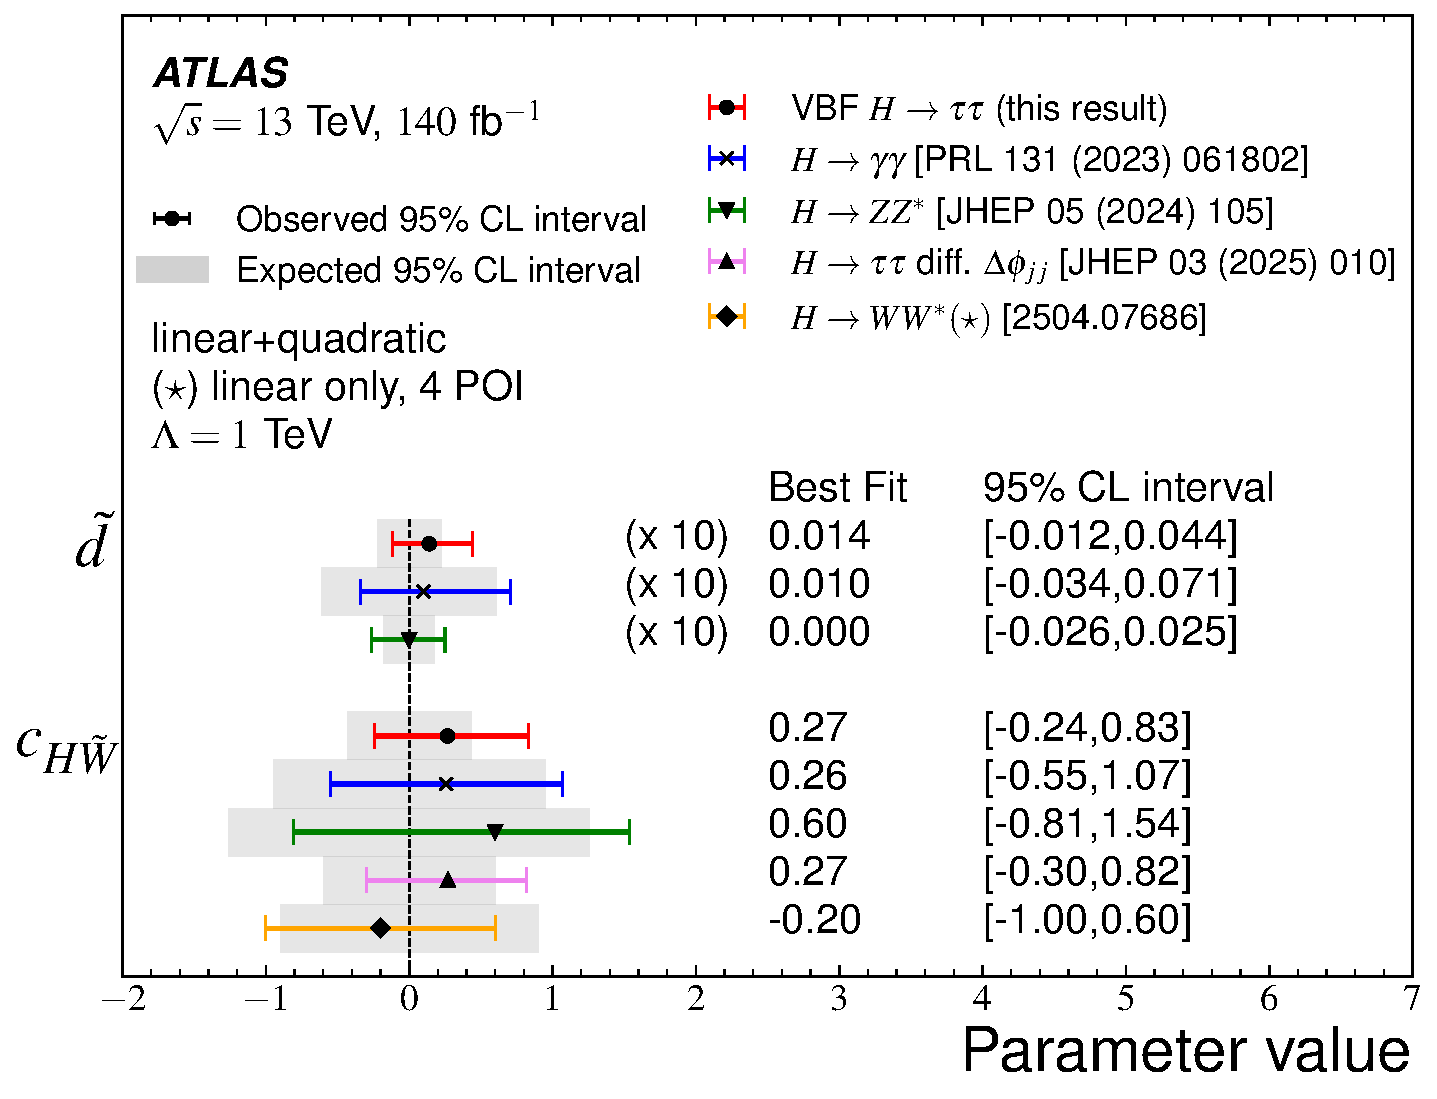
\includegraphics[width=0.45\textwidth]{httcp-atlas}
\caption
    {Left: likelihood scan for the expected and observed constraints
      of the HVV coupling parameter $f_{a3}$, with $p$-value$_{\rm SM}
      = 0.96$ from the CMS anomalous couplings analysis using
      $H\to\gamma\gamma$ decay~\cite{hggac-cms}. Right: comparison of
      results of the present ATLAS $H\to\tau^+\tau^-$ analysis with the $H\to
      ZZ^*\to 4\ell$ analysis $H\to\gamma\gamma$ VBF measurements for
      the CP parameters $c_{H\tilde{W}}$ and $\tilde{d}$.  The data
      points show the observed results, and the uncertainty bands
      correspond to the 95\% CL
      interval~\cite{httcp-atlas}.\label{fig:cp}
    }
\end{figure}


\section{Higgs Boson Pair Production in $b\bar{b}\gamma\gamma$ Final State}

A key goal of the LHC programme and an intense line of current
research is probing the Higgs potential and electroweak symmetry
breaking.  In the SM, the Higgs potential is fully determined by the
vacuum expectation value $v\approx246$ GeV and $m_H\approx125$ GeV.
Deviations from the SM form would signal new physics, with the
trilinear coupling $\kappa_\lambda$ accessible via Higgs pair
production ($HH$).  Gluon-gluon fusion (ggF) and vector-boson fusion
(VBF) are the main $HH$ production modes, with contributions from
$HHH$, $t$-quark Yukawa, $VVH$, and $VVHH$ vertices.  Destructive
interference between diagrams makes sensitivity to $\kappa_\lambda$
largest near the $HH$ production threshold, with cross sections
$\sigma_{HH}^{\rm ggF}\sim30$ fb and $\sigma_{HH}^{\rm VBF}\sim1.7$ fb
at 13 TeV.  A new analysis from ATLAS~\cite{hhbbgg-atlas}, using 140
fb$^{-1}$ of Run-2 and 168 fb$^{-1}$ of Run-3 data, targets the $HH\to
b\bar{b}\gamma\gamma$ channel, which has low branching ratio (0.26\%)
but excellent diphoton mass resolution and high efficiency near
threshold.  Improvements include transformer-based $b$-tagging (GN2)
and a kinematic fit.

The analysis selects events containing exactly two well-reconstructed
photons and at least two $b$-jets candidates.  This selection includes
di-photon triggers, tight photon identification, isolation
requirements, and at least two $b$-tagged jets. Jets are reconstructed
with the anti-$k_t$ algorithm and novel corrections improve the $b\bar{b}$ and
$b\bar{b}\gamma\gamma$ invariant mass resolution by up to 46\%.

Events are categorized into high- and low-mass regions based on the
modified four-body invariant mass
$m^*_{b\bar{b}\gamma\gamma}$. Boosted Decision Trees (BDTs) are used
to separate signal from background, defining exclusive
categories. Signal and background $m_{\gamma\gamma}$ distributions are
modeled analytically, with non-resonant backgrounds estimated using
data-driven methods. Systematic uncertainties arise from photon and
jet calibration, $b$-tagging, luminosity, and theoretical predictions,
while statistical uncertainties dominate.

The measured Higgs pair signal strength is
$\mu_{HH}=0.9^{+1.3}_{-1.0}\text{(stat.)}^{+0.6}_{-0.5}\text{(syst.)}$,
corresponding to a 95\% CL upper limit of $\mu_{HH}<3.8$. Constraints
on the Higgs self-coupling and quartic couplings are $-1.7 <
\kappa_\lambda < 6.6$ and $-0.5 < \kappa_{2V} < 2.6$, respectively,
improving upon previous results. The Fig.~\ref{fig:hhbbgg-atlas} show
the reconstructed diphoton mass for the selected events, with the fit
superimposed, and the observed 95\% CL upper limit on the signal
strength of the process.

\begin{figure}[!tbp]
\centering
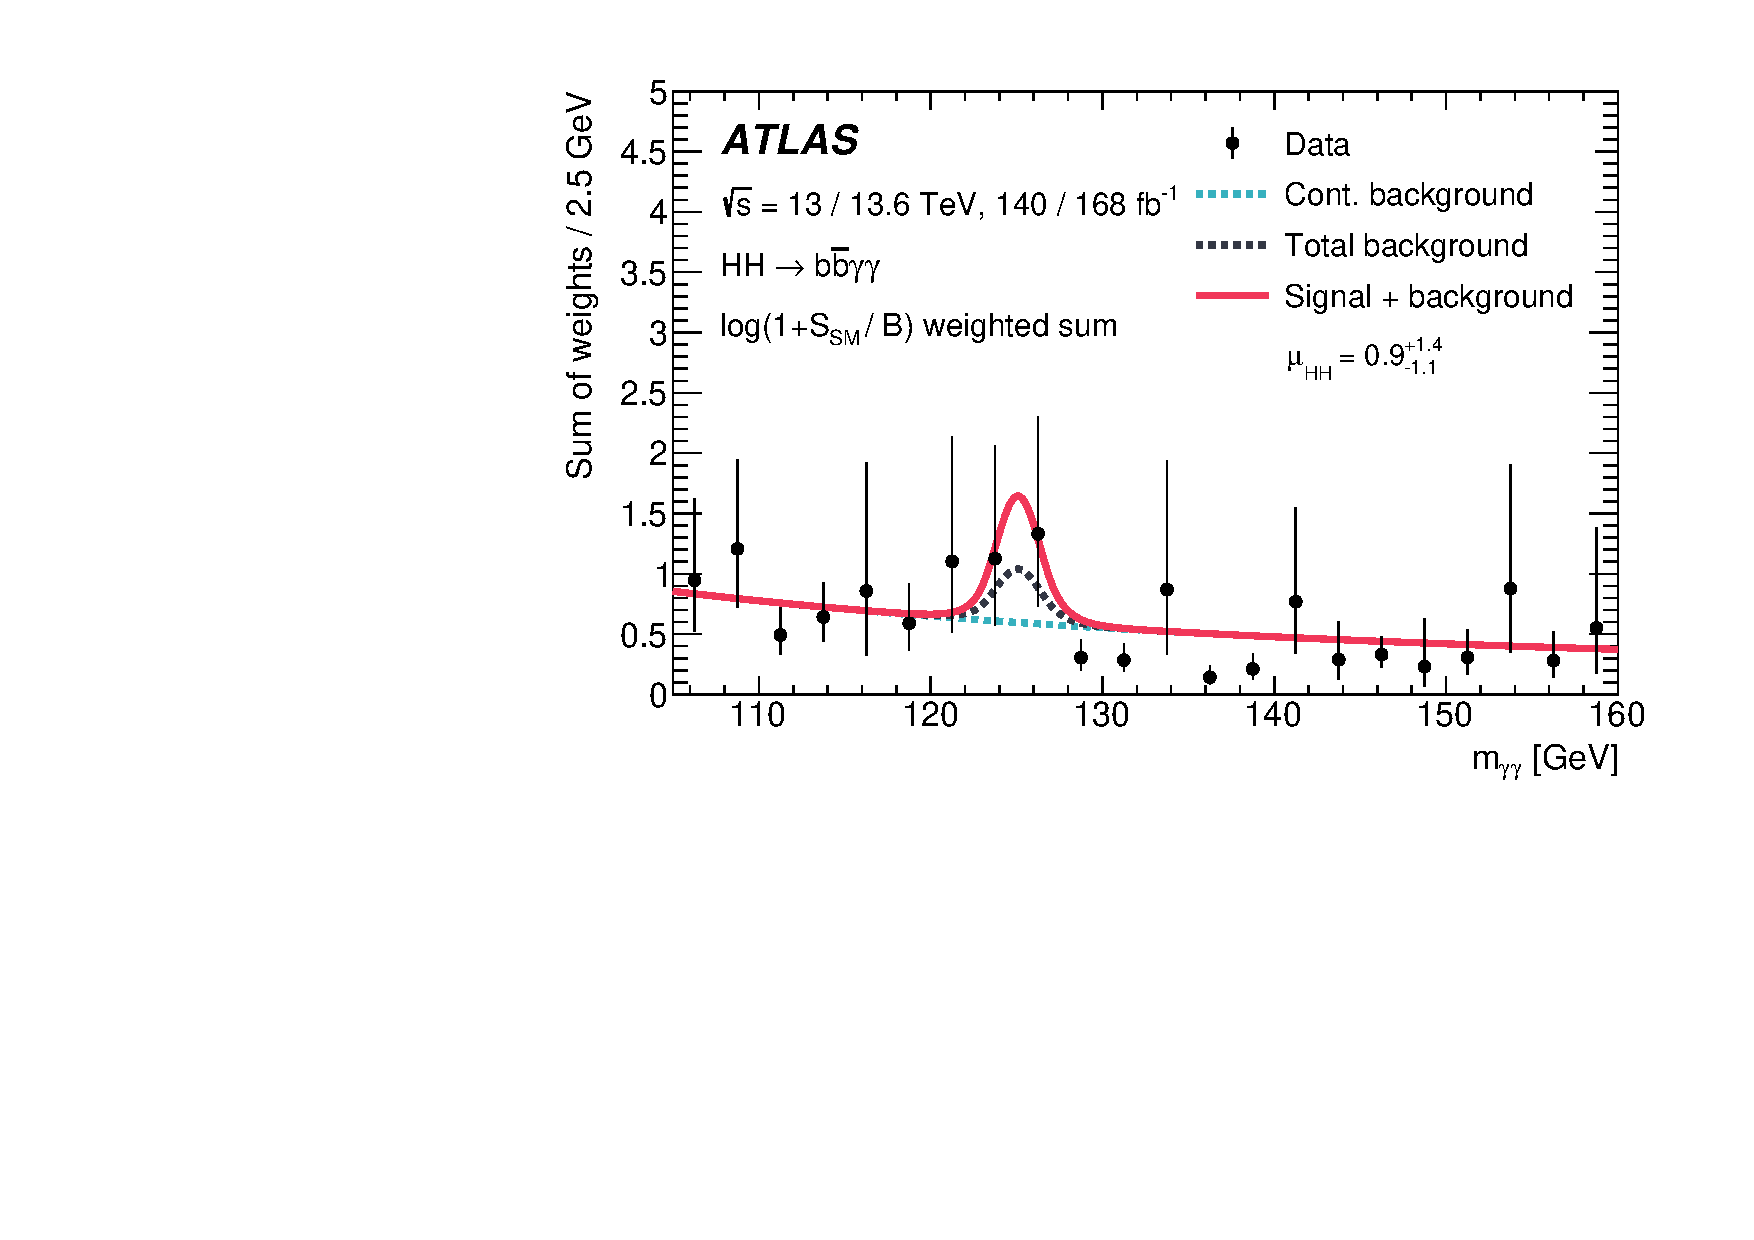
\includegraphics[width=0.45\textwidth]{hhbbgg-mass-atlas}
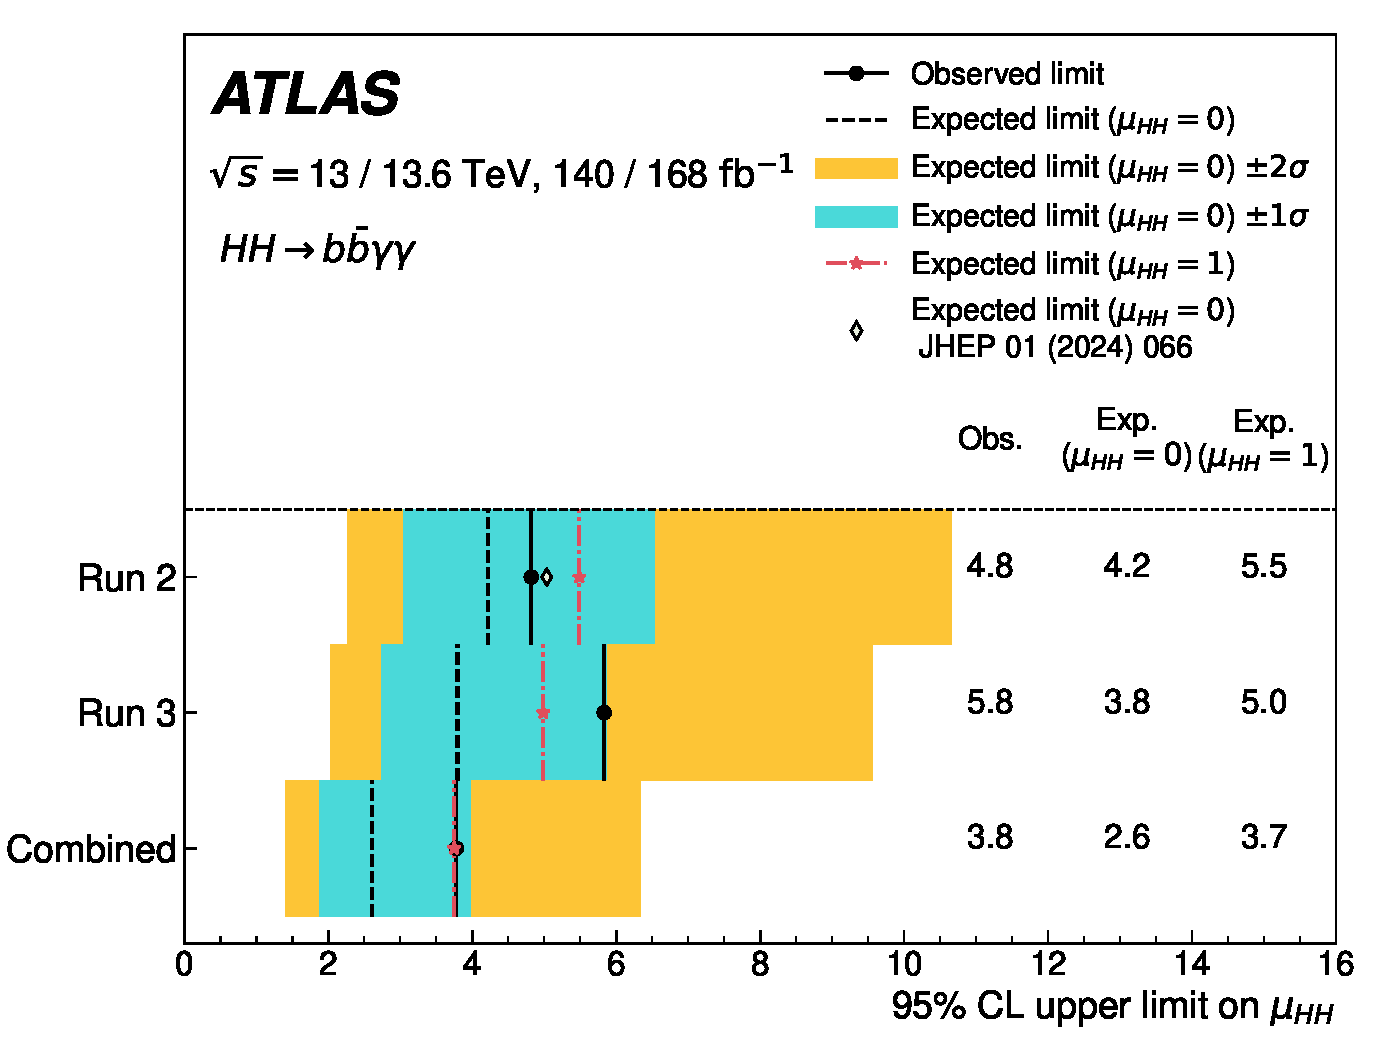
\includegraphics[width=0.45\textwidth]{hhbbgg-ul-atlas}
\caption
    {Left: S/B weighted di-photon invariant mass distribution in
      \SI{308}{fb^{-1}} of ATLAS data, with the superimposed
      likelihood fit. The lines show the fit results for the continuum
      background only (light dotted), adding single Higgs boson
      backgrounds (black dotted) and the full fit (solid). Right:the
      95\% CL upper limits on the $HH\to b\bar b\gamma\gamma$ signal
      strength, obtained with the Run-2 and Run-3 data as well as
      their combination in the ATLAS
      analysis.~\cite{hhbbgg-atlas}.\label{fig:hhbbgg-atlas} }
\end{figure}

\section{Summary}

Recent studies by the ATLAS and CMS collaborations have presented
combinations of measurements of simplified template cross sections,
measurements for the second generation Yukawa couplings, and searches
of rare productions or decay modes for the Higgs boson.  Moreover,
investigations of the CP properties both with verctor bosons or
fermions have been performed. Investigations on the self-coupling of
the Higgs boson, crucial for the determination of the Higgs potential,
have been also performed with increasing precision. These analyses
utilized the full Run 2 dataset and the first part of Run 3 of the
LHC, yielding results consistent with Standard Model expectations.
Ongoing analyses continue to exploit this growing
dataset. Consequently, increasingly precise determinations of Higgs
boson production cross sections and properties are anticipated in the
near future.

\bibliographystyle{JHEP}
\bibliography{dimarco}

\end{document}


